\documentclass{IEEEtran}
\usepackage[spanish]{babel}
\usepackage[utf8]{inputenc}
\usepackage{enumerate}
\usepackage{cite}
\usepackage{graphicx}  
\usepackage{subfig}
\usepackage{float}
\usepackage{tikz}
\usepackage{pgfplots}

\usetikzlibrary{pgfplots.dateplot}
\usepackage{pgfplotstable}
\usepackage{filecontents}
\pgfplotsset{compat=1.15}
% correct bad hyphenation here
\hyphenation{op-tical net-works semi-conduc-tor}


\begin{document}
%
% paper title
% can use linebreaks \\ within to get better formatting as desired
% Do not put math or special symbols in the title.
\title{Práctica: Multiplicación de matrices}


% author names and affiliations
% use a multiple column layout for up to three different
% affiliations
\author{\IEEEauthorblockN{Andrés Fernando Román Arévalo, Ronald Sarmiento\\}
\IEEEauthorblockA{Email:afromana@unal.edu.co, roasarmientoga@unal.edu.co\\}
\IEEEauthorblockA{Universidad Nacional Bogotá, Colombia \\}
}


% make the title area
\maketitle

\nonstopmode

\tableofcontents 
\hfill


\begin{abstract}
El presente informe muestra como se llevo a cabo la paralelización  mediante el uso de distintas plataformas de programación como lo son openMP,CUDA  y openMPI de la multiplicación de matrices.
Para un correcto analisis de los resultados se tuvo en cuenta como metricas tanto el Speed Up como de Time Response 
para los distintos  tamaños de matrices (8,16,32,64,128,256,512 y 1024), de bloques(2,3,4,5,6,7,8,9,10,11,12,13 y 14) y de hilos (10,20,40,60,100,200,400,600,800 y 1000)

\end{abstract}

% no keywords


\IEEEpeerreviewmaketitle



\section{Introducción.}
% no \IEEEPARstart
La multiplicación de matrices es una  de las operaciones  mas basicas que incluso es enseñada en la primaria.
 Pero ha pesar de  su    simplicidad ha sido altamente estudiada en  el campo  de la computación  lo   cual
 ha   hecho que se  desarrollen   algortimos tanto secuenciales como  paralelos para resolver  el problema de 
 una manera  mas optima.  Dentro de estos podemos mencionar el de  Strassen, divide  and conquer, Coppersmith–Winograd entre otros\\\\
% You must have at least 2 lines in the paragraph with the drop letter
% (should never be an issue)
Aun asi paralelizar tiene su limite el cual es explicado en la Ley de Amdahl, la cual establece que hay un punto en que paralelizar ya no ofrece mejoras significativas de rendimiento e incluso por el contrario puede llevar al deterioro del mismo.\\\\


\begin{figure}[H]
  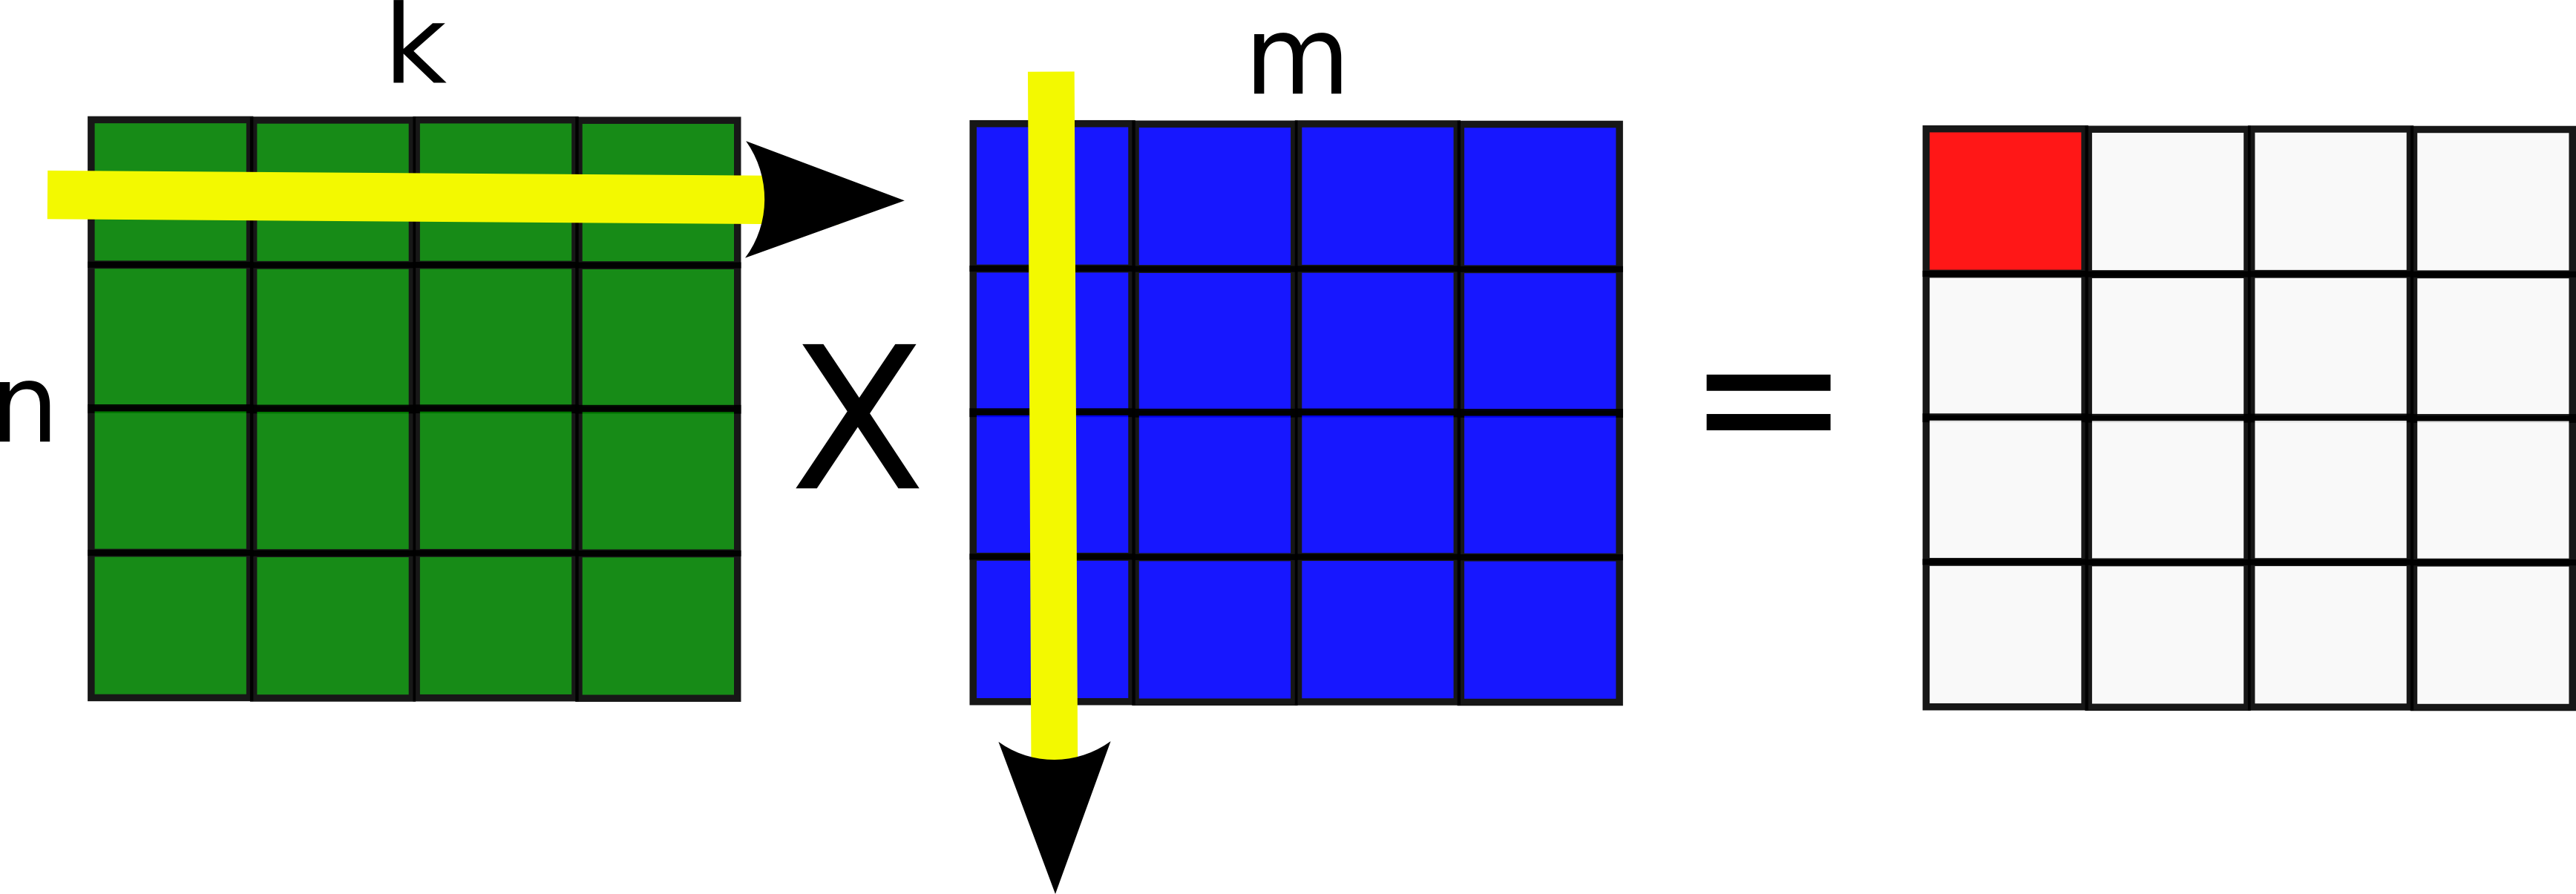
\includegraphics[width=\linewidth]{matrix.png}
  \caption{Multiplicacion matricial}
  \label{fig:boat1}
\end{figure}
\subsection{Multiplicación matricial}

Para esta practica se paralelizo el algoritmo naive de multiplicación de matrices.Donde se tomaron  las matrices
de archivos csv donde  se  prepararon  matrices aleatorias de diferente tamaño. Cabe aclarar que el nombre
indica el tamaño de la matriz. Es decir si el archivo se llama 16A.csv eso quiere decir que es la primera 
matriz y tiene  un  tamaño de  16x16.  

\section{Algoritmo del paralización.}
La paralelizacion se realizo mediante asignación tipo blockwise es decir que se tomo la primera  matriz y se dividio a lo alto en 
filas y a cada una de estas se asigno a un hilo o  bloque. Es decir que un caso hipotetico donde se quiera hacer la multiplicacion 
a dos matrices  de tamaño 16,y   se  lanzan 4 hilos entonces  el hilo 1 se le asignaba la fila 1 a la 4, al 2 la fila 5 a la 8
, al 3 la fila  9 a la  12  y al 4 de  la fila 13 a la 16 . \\\\
Cada hilo  hace  la  multiplicación correspondiente generando en la matriz  producto la  fila que le corresponde

\section{Experimentos y resultados.}
\subsection{POSIX y OpenMP}

Antes de mostrar los resultados obtenidos y compararlos con los que se obtuvieron al paralelizar el efecto difuso con POSIX, es necesario dar a conocer las especificaciones correspondientes del ordenador donde corrio el algoritmo. Para esto se construyo la siguiente tabla resumiendo dicha información:

\begin{table}[H]
\centering
    \begin{tabular}{ |c|c| } 
\hline
\multicolumn{2}{|c|}{Especificaciones} \\
\hline
Modelo & Lenovo G50-45\\
 \hline
 Procesador & AMD A8-6410 / 2 Gz \\ 
 \hline
 Tarjeta gráfica & AMD Radeon R5 \\ 
 \hline
 Nucleos & 4\\ 
 \hline
 Memoria Ram & 8192 MB DDR3
 \\ 
 \hline
 Sistema operativo & Manjaro 18.0.4 \\ 
 \hline
\end{tabular}
\caption{Especificaciones del ordenador}
\end{table}

Para evitar o disminuir posibles interferencias se corrio un script que automaticamente cogio todos los casos de prueba mencionados en el resumen, tambien se busco que no haya ninguna aplicacion abierta mientras se corria el script

\subsubsection{Resultados}
Como primera medida se utilizo el time response o tiempo de ejecución de un programa, donde para cada multiplicación  matricial
 se crearon sus corresponientes gráficas donde en eje horizontal se colocaron el numero de hilos que ejecutaba el programa y en el eje vertical el tiempo que tardo. Para no sobrecargar la gráfica se decidio incluir solo tres tamaños
 de matriz por grafico.\\
A continuacion se presentan las gráficas correspondientes:
\begin{itemize}
    \item \textbf{Matrices de tamaño 8,16 y  32}
    
    \begin{tikzpicture}
\begin{axis}[
xticklabels={},
extra x ticks={1,2,3,4,5,6,7,8,9,10,11,12},
title={Time Response 8,16 y 32},
xlabel={Numero de hilos},
ylabel={Tiempo},
nodes near coords, 
 every node near coord/.append style={font=\tiny,yshift=-1.6pt},
 nodes near coords style={/pgf/number format/.cd,precision=3},
]
\addplot coordinates { (1,0.009) (2,0.008) (3,0.01) (4,0.019) (5,0.01) (6,0.019)  (7,0.009) (8,0.009) (9,0.01) (10,0.009)  (11,0.007)  (12,0.008) };
\addplot coordinates { (1,0.008) (2,0.008) (3,0.02) (4,0.015) (5,0.008) (6,0.008)  (7,0.009) (8,0.021) (9,0.013) (10,0.009)  (11,0.012)  (12,0.02) };
\addplot coordinates { (1,0.011) (2,0.018) (3,0.017) (4,0.012) (5,0.01) (6,0.009)  (7,0.011) (8,0.011) (9,0.021) (10,0.014)  (11,0.009)  (12,0.011) };

\addlegendentry{Size 8}
\addlegendentry{Size 16}
\addlegendentry{Size 32}
\end{axis}
\end{tikzpicture}

Como podemos  observar de la anterior gráfica  el beneficio
de la paralelización en matrices pequeñas no es significativo.
Esto se debe al tiempo de  lanzado   de hilos en estos casos
aun es un tiempo significativo  si lo  comparamos con el tiempo
total que demora el algortimo.

\item \textbf{Matrices de tamaño 256 y 512}

\begin{tikzpicture}
    \begin{axis}[
    xticklabels={},
    extra x ticks={1,2,3,4,5,6,7,8,9,10,11,12},
    title={Time Response 256 y 512},
    xlabel={Numero de hilos},
    ylabel={Tiempo},
    nodes near coords, 
     every node near coord/.append style={font=\tiny,yshift=-1.6pt},
     nodes near coords style={/pgf/number format/.cd,precision=3},
    ]
    \addplot coordinates { (1,0.313) (2,0.209) (3,0.156) (4,0.161) (5,0.175) (6,0.157)  (7,0.142) (8,0.141) (9,0.145) (10,0.158)  (11,0.149)  (12,0.164) };
    \addplot coordinates { (1,2.848) (2,1.550) (3,1.13) (4,1.076) (5,0.965) (6,1.047)  (7,0.955) (8,0.983) (9,0.959) (10,1.102)  (11,0.948)  (12,0.964) };
    
    
    \addlegendentry{Size 256}
    \addlegendentry{Size 512}
    \end{axis}
    \end{tikzpicture}


\item \textbf{Matriz de tamaño 1024}

\begin{tikzpicture}
    \begin{axis}[
    xticklabels={},
    extra x ticks={1,2,3,4,5,6,7,8,9,10,11,12},
    title={Time Response 1024},
    xlabel={Numero de hilos},
    ylabel={Tiempo},
    nodes near coords, 
     every node near coord/.append style={font=\tiny,yshift=-1.6pt},
     nodes near coords style={/pgf/number format/.cd,precision=3},
    ]
    \addplot coordinates { (1,36.389) (2,18.292) (3,13.344) (4,10.989) (5,11.466) (6,11.441)  (7,11.333) (8,11.164) (9,11.314) (10,11.313)  (11,11.373)  (12,11.299) };
    
    \addlegendentry{Size 1024}
    \end{axis}
    \end{tikzpicture}
\end{itemize}

Como podemos ver de las anteriores 2 gráficas el comportamiento de la
 paralelización tiende a ser el esperado en matrices grandes donde el 
 tiempo de  lanzamiento de los hilos  ya no es significante.

Tambien  se  observa que el time response  tiene cierta tendencia a  mejorar conforme se aumenta la cantidad de hilos que son lanzados hasta los 4 hilos, de ahi en adelante la mejora es insignificante y en algunos casos tiende a desmejorar.
Esto se debe a que el computador donde se corrio el código solo tiene 4 nucleos\\

Otra medida que se considero determinar para medir el rendimiento del programa es el speed up es decir el tiempo de ejecución secuencial dividido entre el tiempo de ejecución paralelo. \\
A continuación se presentan las gráficas correspondientes:

\begin{itemize}

    \item \textbf{Matrices de tamaño 8,16 y  32}
    
    \begin{tikzpicture}
\begin{axis}[
xticklabels={},
extra x ticks={1,2,3,4,5,6,7,8,9,10,11,12},
title={ Speed Up 8,16 y 32},
xlabel={Numero de hilos},
ylabel={Tiempo},
nodes near coords, 
 every node near coord/.append style={font=\tiny,yshift=-1.6pt},
 nodes near coords style={/pgf/number format/.cd,precision=3},
 legend pos=south east,
 ]
\addplot coordinates { (2,1.125) (3,0.9) (4,0) (5,0.9) (6,0.474) (7,1)  (8,1) (9,0.9) (10,1) (11,1.286)  (12,1.125) };
\addplot coordinates { (2,1) (3,0.4) (4,0.533) (5,1) (6,1) (7,0.889)  (8,0.381) (9,0.615) (10,0.889) (11,0.667)  (12,0.4) };
\addplot coordinates { (2,0.611) (3,0.647) (4,0.917) (5,1.1) (6,1.222) (7,1)  (8,1) (9,0.524) (10,0.786) (11,1.222)  (12,1) };


\addlegendentry{Size 8}
\addlegendentry{Size 16}
\addlegendentry{Size 32}
\end{axis}
\end{tikzpicture}

    \item \textbf{Matrices de tamaño 256 ,512 y 1024}
    
    \begin{tikzpicture}
        \begin{axis}[
        xticklabels={},
        extra x ticks={1,2,3,4,5,6,7,8,9,10,11,12},
        title={ Speed Up 256,512 y 1024},
        xlabel={Numero de hilos},
        ylabel={Tiempo},
        nodes near coords, 
         every node near coord/.append style={font=\tiny,yshift=-1.6pt},
         nodes near coords style={/pgf/number format/.cd,precision=3},
         legend pos=south east,
         ]
        \addplot coordinates { (2,1.498) (3,2.006) (4,1.944) (5,1.789) (6,1.994) (7,2.204)  (8,2.22) (9,2.159) (10,1.981) (11,2.101)  (12,1.909) };
        \addplot coordinates { (2,1.837) (3,2.52) (4,2.647) (5,2.951) (6,2.720) (7,2.982)  (8,2.897) (9,2.970) (10,2.584) (11,3.004)  (12,2.954) };
        \addplot coordinates { (2,1.989) (3,2.727) (4,3.311) (5,3.174) (6,3.181) (7,3.211)  (8,3.259) (9,3.216) (10,3.217) (11,3.2)  (12,3.221) };
        
        \addlegendentry{Size 256}
        \addlegendentry{Size 512}
        \addlegendentry{Size 1024}
        \end{axis}
        \end{tikzpicture}

    
\end{itemize}

Como podemos observar en las gráficas anteriores el speed up es el esperado ya que el tiempo tiene una tendencia a aumentar conforme el programa se ejecuta con más hilos.\\


\subsection{CUDA}
Antes de mostrar los resultados obtenidos y compararlos con los que se obtuvieron al paralelizar el efecto difuso que se obtuvo con CUDA en comparación con los de CPU(POSIX Y OpenMP), es necesario decir que se corrio en el entorno de Google Colab. 


\subsubsection{Resultados}
Como primera medida se utilizo el time response o tiempo de ejecución de un programa, donde para cada imagen se crearon sus corresponientes gráficas donde en eje horizontal se colocaron el tamaño del kernel que ejecutaba el programa y en el eje vertical el tiempo que tardo.\\
A continuacion se presentan las gráficas correspondientes:
\begin{itemize}
    \item \textbf{Imagen de 720p}
    
    \begin{tikzpicture}
\begin{axis}[
xticklabels={},
extra x ticks={1,2,3,4,5,6,7,8,9,10,11,12,13,14},
title={Time Response 720p},
xlabel={Tamaño del kernel},
ylabel={Tiempo},
nodes near coords, 
 every node near coord/.append style={font=\tiny,yshift=-1.6pt},
 nodes near coords style={/pgf/number format/.cd,precision=3},
]
\addplot coordinates { (2,0.375) (3,0.355) (4,0.420) (4,0.383) (6,0.469) (7,0.396) (8,0.419) (9,0.417) (10,0.494) (11,0.492) (12,0.563) (13,0.560) (14,0.691)};
\end{axis}
\end{tikzpicture}



\item \textbf{Imagen de 1080p}

    \begin{tikzpicture}
\begin{axis}[
xticklabels={},
extra x ticks={1,2,3,4,5,6,7,8,9,10,11,12,13,14},
title={Time Response 1080p},
xlabel={Tamaño del kernel},
ylabel={Tiempo},
nodes near coords, 
 every node near coord/.append style={font=\tiny,yshift=-1.6pt},
 nodes near coords style={/pgf/number format/.cd,precision=3},
]
\addplot coordinates { (2,0.377) (3,0.372) (4,0.441) (4,0.433) (6,0.530) (7,0.526) (8,0.629) (9,0.633) (10,0.848) (11,0.845) (12,1.121) (13,1.128) (14,1.452)};
\end{axis}
\end{tikzpicture}

\item \textbf{Imagen de 4k}

    \begin{tikzpicture}
\begin{axis}[
xticklabels={},
extra x ticks={1,2,3,4,5,6,7,8,9,10,11,12,13,14},
title={Time Response 4k},
xlabel={Tamaño del kernel},
ylabel={Tiempo},
nodes near coords, 
 every node near coord/.append style={font=\tiny,yshift=-1.6pt},
 nodes near coords style={/pgf/number format/.cd,precision=3},
]
\addplot coordinates { (2,1.391) (3,1.397) (4,1.717) (5,1.734) (6,2.240) (7,2.237) (8,2.9) (9,2.898) (10,3.833) (11,3.830) (12,4.755) (13,4.768) (14,6.078)};
\end{axis}
\end{tikzpicture}


\end{itemize}

Como se puede observar en las gráficas anteriores el time response del código tiene cierta tendencia de  empeorar  conforme se aumenta el tamaño del kernel, como es el comportamiento esperado.\\
Otra medida que se considero determinar para medir el rendimiento de los hilos en el programa es el speed up que para este caso se calculo como la división entre el mejor tiempo en CPU contra con los mejores tiempos en GPU \\
A continuación se presentan las gráficas correspondientes:

\begin{itemize}
\item \textbf{Imagen de 720p}
    
\begin{tikzpicture}
\begin{axis}[
xticklabels={},
extra x ticks={4,6,8,10,12,14},
title={Speed Up 720p},
xlabel={Tamaño del kernel},
ylabel={Tiempo},
nodes near coords, 
 every node near coord/.append style={font=\tiny,yshift=-1.6pt},
 nodes near coords style={/pgf/number format/.cd,precision=3},
 legend pos=south east,
]
\addplot coordinates { (4,0.690) (6,0.978) (8,1.480) (10,1.721) (12,2) (14,2.225) };
\addplot coordinates { (4,1.480) (6,1.837) (8,2.02) (10,2.225) (12,2.467) (14,2.787) };
\addlegendentry{Speed Up GPU-CPU}
\addlegendentry{Speed Up CPU-CPU}
\end{axis}
\end{tikzpicture}
 
 \item \textbf{Imagen de 1080p}  
 
 \begin{tikzpicture}
\begin{axis}[
xticklabels={},
extra x ticks={4,6,8,10,12,14},
title={Speed Up 1080p},
xlabel={Tamaño del kernel},
ylabel={Tiempo},
nodes near coords, 
 every node near coord/.append style={font=\tiny,yshift=-1.6pt},
 nodes near coords style={/pgf/number format/.cd,precision=3},
 legend pos=south east,
]
\addplot coordinates { (4,1.245) (6,1.689) (8,2.130) (10,2.304) (12,2.408) (14,2.470) };
\addplot coordinates { (4,1.779) (6,2.277) (8,2.562) (10,2.772) (12,2.921) (14,2.955) };
\addlegendentry{Speed Up GPU-CPU}
\addlegendentry{Speed Up CPU-CPU}
\end{axis}
\end{tikzpicture}

\item \textbf{Imagen de 4k}

 \begin{tikzpicture}
\begin{axis}[
xticklabels={},
extra x ticks={4,6,8,10,12,14},
title={Speed Up 4k},
xlabel={Tamaño del kernel},
ylabel={Tiempo},
nodes near coords, 
 every node near coord/.append style={font=\tiny,yshift=-1.6pt},
 nodes near coords style={/pgf/number format/.cd,precision=3},
 legend pos=north west,
]
\addplot coordinates { (4,2.889) (6,4.140) (8,5.238) (10,5.978) (12,6.766) (14,6.467) };
\addplot coordinates { (4,2.256) (6,2.622) (8,2.850) (10,2.98) (12,3.055) (14,3.144) };
\addlegendentry{Speed Up GPU-CPU}
\addlegendentry{Speed Up CPU-CPU}
\end{axis}
\end{tikzpicture}

\end{itemize}

\subsection{OpenMPI}
Para esta practica se utilizo 2 clausters, uno que fue creado en google cloud el cual tiene 5 maquinas con las mismas configuraciones es decir con 7.5 gb de ram y 2 vcpu y otro en microsoft azure con 3.5 gb de ram y 1 solo vcpu. El algoritmo para distribuir entre maquinas utiliza MPI indicando un proceso por cada máquina del cluster(5 máquinas) y variando el numero de hilos por máquina(1 - 10) .  Se corrió el algoritmo y se sacaron las siguientes gráficas en el caso del time response:

\begin{itemize}
\item \textbf{Imagen de 720p}


\begin{tikzpicture}
\begin{axis}[
xticklabels={},
extra x ticks={1,2,3,4,5,6,7,8,9,10},
title={Time Response 720p},
xlabel={Numero de hilos},
ylabel={Tiempo},
nodes near coords, 
every node near coord/.append style={font=\tiny,yshift=-1.6pt},
    nodes near coords style={/pgf/number format/.cd,precision=3},
]
\addplot coordinates { (1,1.251) (2,1.256) (3,1.252) (4,1.215) (5,1.234) (6,1.242) (7,1.243) (8,1.238) (9,1.228) (10,1.235) };
\addplot coordinates { (1,1.238) (2,1.220) (3,1.229) (4,1.258) (5,1.213) (6,1.252) (7,1.225) (8,1.214) (9,1.24) (10,1.227) };
\addplot coordinates { (1,1.250) (2,1.260) (3,1.242) (4,1.253) (5,1.269) (6,1.294) (7,1.243) (8,1.266) (9,1.276) (10,1.251) };
\addlegendentry{Kernel 4}
\addlegendentry{Kernel 6}
\addlegendentry{Kernel 8}
\end{axis}
\end{tikzpicture}

\item \textbf{Imagen de 1080p}


\begin{tikzpicture}
\begin{axis}[
xticklabels={},
extra x ticks={1,2,3,4,5,6,7,8,9,10},
title={Time Response 1080p},
xlabel={Numero de hilos},
ylabel={Tiempo},
nodes near coords, 
every node near coord/.append style={font=\tiny,yshift=-1.6pt},
    nodes near coords style={/pgf/number format/.cd,precision=3},
]
\addplot coordinates { (1,1.281) (2,1.290) (3,1.295) (4,1.285) (5,1.276) (6,1.251) (7,1.27) (8,1.268) (9,1.212) (10,1.306) };
\addplot coordinates { (1,1.354) (2,1.336) (3,1.389) (4,1.355) (5,1.338) (6,1.374) (7,1.326) (8,1.341) (9,1.311) (10,1.276) };
\addplot coordinates { (1,1.520) (2,1.421) (3,1.466) (4,1.388) (5,1.443) (6,1.428) (7,1.409) (8,1.408) (9,1.35) (10,1.316) };

\addlegendentry{Kernel 4}
\addlegendentry{Kernel 6}
\addlegendentry{Kernel 8}
\end{axis}
\end{tikzpicture}


\item \textbf{Imagen de 4k}


\begin{tikzpicture}
\begin{axis}[
xticklabels={},
extra x ticks={1,2,3,4,5,6,7,8,9,10},
title={Time Response 4k},
xlabel={Numero de hilos},
ylabel={Tiempo},
nodes near coords, 
every node near coord/.append style={font=\tiny,yshift=-1.6pt},
    nodes near coords style={/pgf/number format/.cd,precision=3},
]
\addplot coordinates { (1,2.562) (2,2.601) (3,2.55) (4,2.568) (5,2.276) (6,2.246) (7,2.303) (8,2.281) (9,2.241) (10,2.246) };
\addplot coordinates { (1,3.151) (2,3.081) (3,3.122) (4,3.056) (5,2.832) (6,2.794) (7,2.797) (8,2.801) (9,2.81) (10,2.818) };
\addplot coordinates { (1,3.905) (2,4.060) (3,3.984) (4,3.962) (5,3.685) (6,3.677) (7,3.648) (8,3.647) (9,3.674) (10,3.718	) };

\addlegendentry{Kernel 4}
\addlegendentry{Kernel 6}
\addlegendentry{Kernel 8}
\end{axis}
\end{tikzpicture}




\end{itemize}

Al momento de graficar el speed up se comparo el de la anterior practica que fue la de CUDA con el speed up de la practica actual.  Es decir se hizo la comparación entre GPU-CPU, CPU-CPU, 1 vcpu y  2 vcpu. Las  gráficas obtenidas para los diferentes tamaños de imagenes se muestran a continuación:

\begin{itemize}
\item \textbf{Imagen de 720p}


\begin{tikzpicture}
\begin{axis}[
xticklabels={},
extra x ticks={4,6,8,10,12,14},
title={Speed Up 720p},
legend pos= north west,
xlabel={Tamaño del kernel},
ylabel={Speed Up},
]
\addplot+[nodes near coords, 
every node near coord/.append style={font=\tiny,yshift=-1.6pt},
    nodes near coords style={/pgf/number format/.cd,precision=3},] coordinates { (4,0.690) (6,0.9782) (8,1.4797) (10,1.7206) (12,2) (14,2.2547)};
\addplot+[nodes near coords, 
every node near coord/.append style={font=\tiny,yshift=-1.6pt},
    nodes near coords style={/pgf/number format/.cd,precision=3},] coordinates { (4,1.4795) (6,1.8367) (8,2.0195) (10,2.2251) (12,2.4667) (14,2.7871)};
\addplot+[nodes near coords, 
every node near coord/.append style={font=\tiny,yshift=-1.6pt},
    nodes near coords style={/pgf/number format/.cd,precision=3},] coordinates { (4,0.1578) (6,0.1956) (8,0.2372) (10,0.2846) (12,0.3254) (14,0.4497)  };
\addplot coordinates { (4,0.1321) (6,0.165) (8,0.2168) (10,0.2596) (12,0.3074) (14,0.3670)  };

\addlegendentry{GPU-CPU}
\addlegendentry{CPU-CPU}
\addlegendentry{1vcpu}
\addlegendentry{2vcpu}

\end{axis}
\end{tikzpicture} 

\item \textbf{Imagen de 1080p}


\begin{tikzpicture}
\begin{axis}[
xticklabels={},
extra x ticks={4,6,8,10,12,14},
title={Speed Up 1080p},
legend style={at={(0.97,0.5)},anchor=east},
xlabel={Tamaño del kernel},
ylabel={Speed Up},
]
\addplot+[nodes near coords, 
every node near coord/.append style={font=\tiny,yshift=-1.6pt},
    nodes near coords style={/pgf/number format/.cd,precision=3},] coordinates { (4,1.2448) (6,1.6887) (8,2.1303) (10,2.3042) (12,2.4077) (14,2.4704)};
\addplot+[nodes near coords, 
every node near coord/.append style={font=\tiny,yshift=-1.6pt},
    nodes near coords style={/pgf/number format/.cd,precision=3},] coordinates { (4,1.7789) (6,2.2773) (8,2.5621) (10,2.7716) (12,2.921) (14,2.9546)};
\addplot+[nodes near coords, 
every node near coord/.append style={font=\tiny,yshift=-1.6pt},
    nodes near coords style={/pgf/number format/.cd,precision=3},] coordinates { (4,0.2320) (6,0.308) (8,0.3974) (10,0.4982) (12,0.6123) (14,0.7192)  };
\addplot coordinates { (4,0.2085) (6,0.2540) (8,0.3283) (10,0.4448) (12,0.5837) (14,0.6989) };

\addlegendentry{GPU-CPU}
\addlegendentry{CPU-CPU}
\addlegendentry{1vcpu}
\addlegendentry{2vcpu}

\end{axis}
\end{tikzpicture} 


\item \textbf{Imagen de 4k}


\begin{tikzpicture}
\begin{axis}[
xticklabels={},
extra x ticks={4,6,8,10,12,14},
title={Speed Up 4k},
legend style={at={(0.97,0.62)},anchor=east},
xlabel={Tamaño del kernel},
ylabel={Speed Up},
]
\addplot+[nodes near coords, 
every node near coord/.append style={font=\tiny,yshift=-1.6pt},
    nodes near coords style={/pgf/number format/.cd,precision=3},] coordinates { (4,2.889) (6,4.14) (8,5.238) (10,5.978) (12,6.766) (14,6.467)};
\addplot+[nodes near coords, 
every node near coord/.append style={font=\tiny,yshift=-1.6pt},
    nodes near coords style={/pgf/number format/.cd,precision=3},] coordinates { (4,2.2562) (6,2.6224) (8,2.8499) (10,2.98) (12,3.0548) (14,3.1437)};
\addplot coordinates { (4,0.9509) (6,1.2642) (8,1.46101) (10,1.668) (12,1.856) (14,1.9795)  };
\addplot+[nodes near coords, 
every node near coord/.append style={font=\tiny,yshift=-1.6pt},
    nodes near coords style={/pgf/number format/.cd,precision=3},] coordinates { (4,1.028) (6,1.4223) (8,1.7802) (10,2.0917) (12,2.2979) (14,2.5181) };

\addlegendentry{GPU-CPU}
\addlegendentry{CPU-CPU}
\addlegendentry{1vcpu}
\addlegendentry{2vcpu}

\end{axis}
\end{tikzpicture} 




\end{itemize}


\section{Conclusiones}
\begin{enumerate}
    \item POSIX y OpemMP
            \begin{itemize}
          \item Entre mas grande es el kernel con el que se trabaja se demora un tiempo superior en realizar el efecto difuminado debido a que realiza mas operaciones al momento de calcular el promedio del kernel, haciendo que el costo computacional sea superior
          \item Como se observa en los resultados presentados en las tablas anteriores la mejora solo se aprecia que es significativa hasta los 4 hilos y considero que se debe a que el procesador donde se corrio el código  solo posee 4
          nucleos
          \item Aunque la diferencia entre el uso de POSIX y OpenMP podria parecer muy pequeña en realidad al momento de hacer un gran conjunto de  operaciónes tipo  difuminado esta puede ser considerable. Tambien hay que considerar que el algoritmo a nuestra consideración esta bastante optimizado como para que haya una diferencia mayor entre el uso de POSIX y OpenMP
        \end{itemize}
         
    \item CUDA
    
         \begin{itemize}
          \item Entre mas grande es el kernel con el que se trabaja se demora un tiempo superior en realizar el efecto difuminado debido a que realiza mas operaciones al momento de calcular el promedio del kernel, haciendo que el costo computacional sea superior
          \item Se evidencia que el speedup de GPU es menor cuando el computo a realizar es considerablemente menor, ya que es necesario tener en cuenta los tiempos de copia de los datos a calcular en el device y luego la recepcion en host, además que para la implementacion en cuestión es necesario realizar una transformacion de matrizde OpenCV a arreglo de enteros.
          \item Es necesario realizar una comparacion de las implementaciones de CPU y GPU para reconocer cual tiene mejor rendimiento, para nuestra práctica solo vale la pena usar GPU en el computo de imagenes 4K.
        \end{itemize} 
    \item OpenMPI
\end{enumerate}
    \begin{itemize}
        \item Los equipos que computan el problema son maquinas virtuales que están asignadas por google cloud, esto no necesariamente implica que las maquinas son contiguas en una LAN, lo que se asegura es que hacen parte de una misma VLAN lo cual impacta en el desempeño. 
          \item Asegurar que todas las maquinas en el cluster tienen las mismas librerias instaladas no siempre puede ser trivial, lo cual dificulta la implementación.
          \item al igual que en GPU la aceleracion aumenta en la medida que el tiempo de cómputo es cosiderablemente mayor al tiempo de transporte de la información.
          \item La grafica de speedup sufre un cambio similar al de la implementación en GPU, pero ya que la aceleracion es pequeña en comparación no es tan notoria la pendiente positiva.
          \item Es evidente que existe una aceleración de los tiempos de respuesta con respecto a la mejor implementación paralela en una sola máquina, sin embargo aun no se iguala la velocidad que alcanzó la implementación en una GPU.
    \end{itemize}

\noindent 


\begin{thebibliography}{00}
\bibitem{b2} Pedraza, C. (2019). Diapositivas de clase.
\bibitem{b1}David, K. and Wen-Mei, H. (2010). Programming massively parallel processos. 2nd ed. Morgan Kaufmann.
\bibitem{b2} Thomas, R. and Gudula, R. (2010). Parallel Programming. 1st ed. Springer.
\bibitem{b2} En.wikipedia.org. $(2019). Box blur.  Available at: https://en.wikipedia.org/wiki/Box_blur.$
\end{thebibliography}




% that's all folks
\end{document}


